% Native-size vector artwork: 7.055 in x 4.4 in.
% Schematic explanation of the current input-output emulation theorem.
\RequirePackage{fix-cm}
\documentclass[tikz,border=0pt]{standalone}
\usepackage[T1]{fontenc}
\usepackage{helvet}
\usepackage{amsmath,amssymb}
\usetikzlibrary{arrows.meta,calc,decorations.pathreplacing}
\renewcommand{\familydefault}{\sfdefault}
\pdfinfoomitdate=1
\pdftrailerid{}
\pdfsuppressptexinfo=15
\definecolor{ink}{HTML}{202A35}
\definecolor{muted}{HTML}{606C78}
\definecolor{border}{HTML}{C4CED7}
\definecolor{blue}{HTML}{2769B0}
\definecolor{teal}{HTML}{138A83}
\definecolor{orange}{HTML}{D57525}
\begin{document}
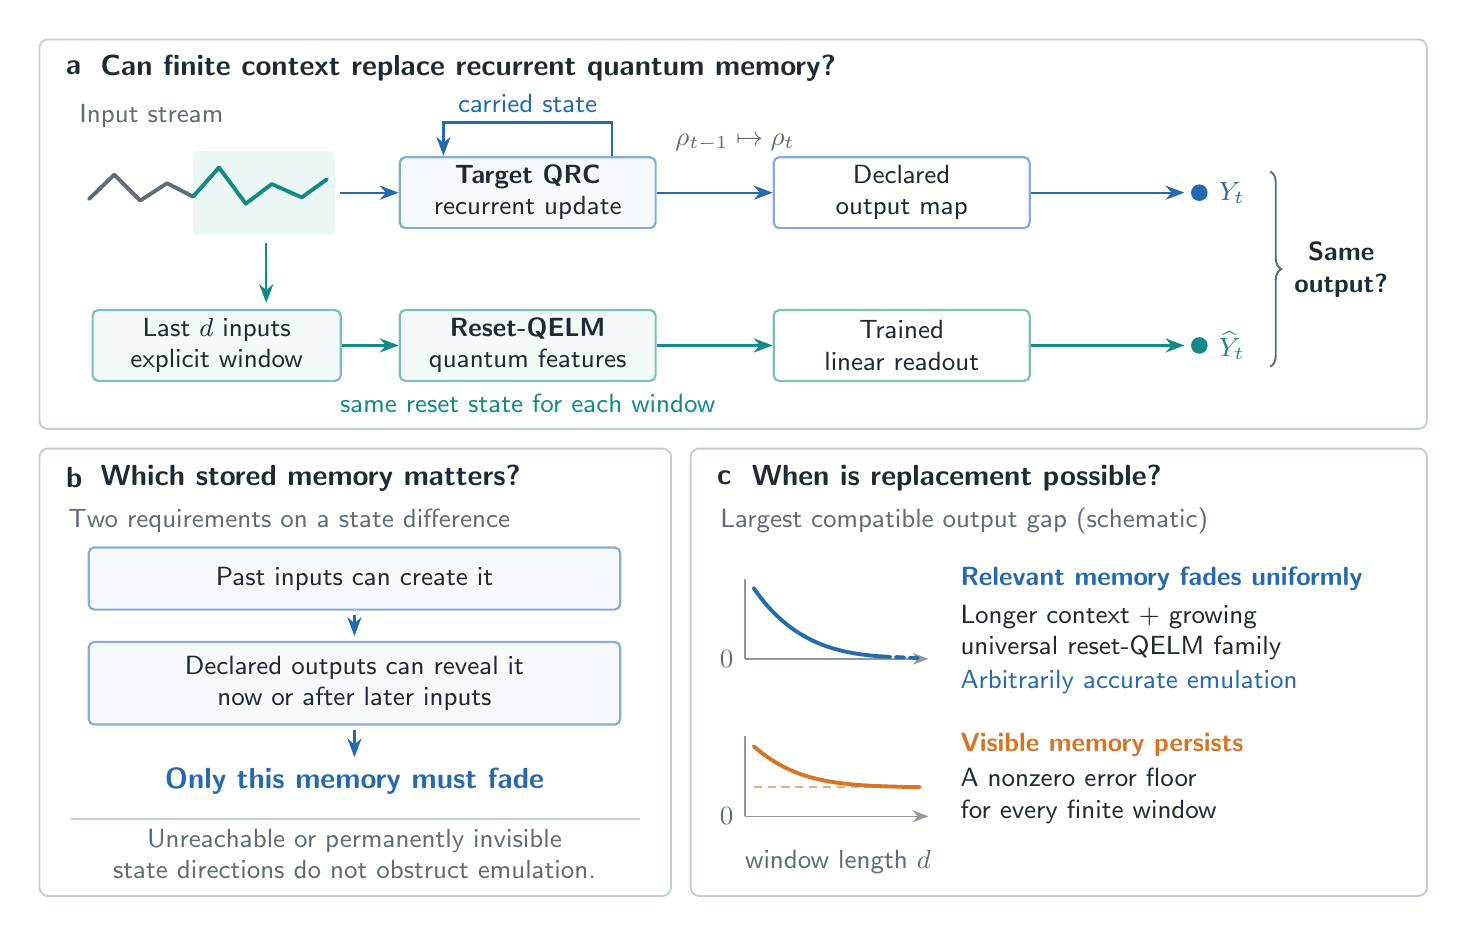
\begin{tikzpicture}[
 x=1cm,y=1cm,
 every node/.style={font=\fontsize{9.5}{11.3}\selectfont,text=ink,inner sep=0pt},
 >={Stealth[length=4.4pt,width=3.4pt]},
 flow/.style={line width=.85pt,draw=muted,-{Stealth}},
 frame/.style={draw=border,line width=.7pt,rounded corners=3pt},
 heading/.style={font=\fontsize{10.5}{12.4}\selectfont\bfseries,anchor=west},
 block/.style={line width=.8pt,rounded corners=2pt,minimum height=.9cm,
               minimum width=3.25cm,align=center,draw=blue!55,fill=blue!4},
 mini/.style={line width=1.4pt,line cap=round,line join=round}
]
\path[use as bounding box] (0,0) rectangle (17.9197,11.176);

% a: two architectures, one declared input-output behavior.
\draw[frame] (.15,6.08) rectangle (17.77,11.026);
\node[heading] at (.48,10.66) {a};
\node[heading] at (.92,10.66) {Can finite context replace recurrent quantum memory?};
\node[anchor=west,text=muted] at (.65,10.05) {Input stream};
\fill[teal!8,rounded corners=2pt] (2.1,8.54) rectangle (3.9,9.61);
\draw[mini,muted] (.78,9.0)--(1.1,9.31)--(1.43,8.98)--(1.77,9.20)--(2.1,9.03);
\draw[mini,teal] (2.1,9.03)--(2.43,9.40)--(2.77,8.94)--(3.1,9.19)--(3.48,9.02)--(3.80,9.25);
\node[block] (qrc) at (6.35,9.08) {\textbf{Target QRC}\\recurrent update};
\node[block,fill=white] (qread) at (11.1,9.08) {Declared\\output map};
\draw[flow,blue] (3.97,9.08)--(qrc.west);
\draw[flow,blue] (qrc.east)--(qread.west);
\draw[flow,blue] (qread.east)--(14.69,9.08);
\fill[blue] (14.88,9.08) circle(3pt);
\node[anchor=west,text=blue] at (15.12,9.08) {$Y_t$};
% Reuse the state, not the measurement record.
\draw[flow,blue] (7.42,9.55)--(7.42,9.97)--(5.28,9.97)--(5.28,9.55);
\node[text=blue] at (6.35,10.22) {carried state};
\node[anchor=west,text=muted] at (8.22,9.72) {$\rho_{t-1}\mapsto\rho_t$};

\draw[flow,teal] (3.03,8.44)--(3.03,7.68);
\node[block,draw=teal!55,fill=teal!5,minimum width=3.15cm] (win) at (2.4,7.14)
 {Last $d$ inputs\\explicit window};
\node[block,draw=teal!55,fill=teal!5] (qelm) at (6.35,7.14)
 {\textbf{Reset-QELM}\\quantum features};
\node[block,draw=teal!55,fill=white] (eread) at (11.1,7.14)
 {Trained\\linear readout};
\draw[flow,teal] (win.east)--(qelm.west);
\draw[flow,teal] (qelm.east)--(eread.west);
\draw[flow,teal] (eread.east)--(14.69,7.14);
\fill[teal] (14.88,7.14) circle(3pt);
\node[anchor=west,text=teal] at (15.12,7.14) {$\widehat Y_t$};
\node[text=teal] at (6.35,6.41) {same reset state for each window};
\draw[muted,line width=.7pt,decorate,decoration={brace,amplitude=4pt}]
 (15.78,9.35)--(15.78,6.87);
\node[align=center,anchor=west,font=\fontsize{9.5}{11.3}\selectfont\bfseries]
 at (16.08,8.10) {Same\\output?};

% b: relevant memory, not indiscriminate full-state contraction.
\draw[frame] (.15,.15) rectangle (8.17,5.83);
\node[heading] at (.48,5.46) {b};
\node[heading] at (.92,5.46) {Which stored memory matters?};
\node[anchor=west,text=muted] at (.51,4.91) {Two requirements on a state difference};
\node[block,minimum width=6.75cm,minimum height=.79cm] (written) at (4.15,4.18)
 {Past inputs can create it};
\draw[flow,blue] (4.15,3.72)--(4.15,3.45);
\node[block,minimum width=6.75cm,minimum height=1.05cm] (visible) at (4.15,2.85)
 {Declared outputs can reveal it\\now or after later inputs};
\draw[flow,blue] (4.15,2.26)--(4.15,1.91);
\node[text=blue,font=\fontsize{10.5}{12.4}\selectfont\bfseries]
 at (4.15,1.60) {Only this memory must fade};
\draw[border,line width=.6pt] (.55,1.13)--(7.78,1.13);
\node[align=center,text=muted] at (4.15,.68)
 {Unreachable or permanently invisible\\state directions do not obstruct emulation.};

% c: largest compatible output gap; both curves are schematic.
\draw[frame] (8.42,.15) rectangle (17.77,5.83);
\node[heading] at (8.75,5.46) {c};
\node[heading] at (9.19,5.46) {When is replacement possible?};
\node[anchor=west,text=muted] at (8.79,4.91)
 {Largest compatible output gap (schematic)};
\foreach \base in {3.16,1.16}{
 \draw[muted!70,line width=.6pt,-{Stealth}] (9.11,\base)--(11.44,\base);
 \draw[muted!70,line width=.6pt] (9.11,\base)--(9.11,{\base+1.02});
 \node[anchor=east,text=muted] at (8.97,\base) {$0$};
}
\draw[mini,blue] (9.22,4.06) .. controls (9.71,3.34) and (10.31,3.23) .. (10.85,3.19);
\draw[mini,blue,densely dashed] (10.85,3.19)--(11.32,3.17);
\node[anchor=west,text=blue,font=\fontsize{9.5}{11.3}\selectfont\bfseries]
 at (11.84,4.17) {Relevant memory fades uniformly};
\node[anchor=west,align=left] at (11.84,3.50)
 {Longer context + growing\\universal reset-QELM family};
\node[anchor=west,text=blue] at (11.84,2.87) {Arbitrarily accurate emulation};

\draw[orange!60,line width=.7pt,densely dashed] (9.22,1.53)--(11.33,1.53);
\draw[mini,orange] (9.22,2.05) .. controls (9.78,1.56) and (10.36,1.55) .. (11.33,1.53);
\node[anchor=west,text=orange,font=\fontsize{9.5}{11.3}\selectfont\bfseries]
 at (11.84,2.07) {Visible memory persists};
\node[anchor=west,align=left] at (11.84,1.42)
 {A nonzero error floor\\for every finite window};
\node[text=muted] at (10.29,.58) {window length $d$};
\end{tikzpicture}
\end{document}
